\documentclass[12pt,parskip=full]{scrartcl}
\usepackage[utf8]{inputenc}   % UTF8-Kodierung für Umlaute
\usepackage{ngerman}          % deutsche Silbentrennung
\usepackage[T1]{fontenc}	  % wichtig für Trennung von Wörtern mit Umlauten
\usepackage{microtype}		  % verbesserter Randausgleich
\usepackage{graphicx}         % Einbindung von Grafiken
\usepackage{wrapfig}			% Grafiken im Text
\usepackage{subcaption}         % Für Subgrafiken
\clubpenalty = 10000           % Keine "Schusterjungen"
\widowpenalty = 10000          % Keine "Hurenkinder"

\title{Ausführliche Nähanleitung Mund-Nasen-Schutz mit Nackenband}
\author{Anna Klingauf}
\date{Oktober 2020}

\begin{document}
\begin{titlepage}
\maketitle
\thispagestyle{empty}
\begin{figure}[b!] 
  \centering
     \includegraphics[width=0.60\textwidth]{Pictures/00_Completed/Gesamt.png}
\end{figure}
\end{titlepage}
\clearpage

\section*{Allgemeines}
Der Mund-Nasen-Schutz (abgekürzt MNS oder Maske) wie er hier vorgestellt wird besteht aus zwei Lagen Baumwollstoff. Im Gegensatz zu den meisten anderen MNS wird er nicht an den Ohren befestigt sondern mit einem elastischen Band im Nacken. Das Band kann mit Klett, Knöpfen oder Druckknöpfen geschlossen werden. Wenn die Maske gerade nicht benötigt wird, kann sie bequem um den Hals getragen werden (Bild am Ende der Anleitung). An der Nase ist sowohl ein Drahteinsatz als auch eine Abdichtung mit Gummi angebracht. Da die Maske durch die Form und die Abdichtung an der Nase sehr dicht ist, beschlägt bei allen bisherigen Testpersonen die Brille auch bei kaltem Wetter nicht. Die Faltung der Maske kann beim Nähen individuell an das Gesicht angepasst werden. Bei den hier vorgestellten Materialien kann die Maske nach ersten Versuchen auch problemlos in der Waschmaschine gewaschen oder ausgekocht werden. Es werden drei Größen als Vorschläge zur Verfügung gestellt, die auch individuell angepasst werden können. \par

Die vorliegende Anleitung soll auch für Anfänger benutzbar sein, deswegen werden zum Einstieg ein paar grundlegende Vorgehensweisen erklärt und bei späteren Schritten viele Fotos zur Verfügung gestellt.

\subsection*{Feststecken}
Bei allen Schritten werden die Stoffstücke hier vor dem Festnähen zuerst mit Stecknadeln aneinander fixiert. Dabei ist das Vorgehen immer gleich: Die Stecknadeln werden in ca. 1-2 cm Abstand voneinander in den Stoff gesteckt, im rechten Winkel zur geplanten Naht. Danach kann man einfach über die Stecknadeln drüber nähen. Dazu sollten die Nadeln aber so gesteckt werden, dass das Füßchen der Nähmaschine nicht an den Köpfen der Stecknadeln hängen bleibt.

\subsection*{Nähte}
Bei allen Nähten die hier beschrieben werden, müssen natürlich die Enden der Fäden vernäht und dann passend abgeschnitten werden. Das Vernähen kann man bei den meisten Nähmaschinen mit den Rückwärts-Hebel erledigen, indem man am Anfang und am Ende einer Naht einmal kurz zurück und dann wieder vorwärts näht. Das Feststecken und Nähte setzen sollte man bei Bedarf vorher an überzähligen Stoffstücken üben.

\section*{Materialien}
Folgende Materialien werden benötigt:
\begin{itemize}
    \item Außenstoff (2 mal ca. 17 x 19 cm), z.B Baumwolle
    \item Innenstoff (2 mal ca. 17 x 19 cm), z.B. Baumwolle
    \item Rest-Stoff (für Drahteinsatz, ca 4 x 10 cm)
    \item 2 Büroklammern, am besten mit Plastiküberzug
    \item Abdichtung, ca. 7 cm, z.B. aus halterlosen Strümpfen
    \item elastisches Band, ca. 45 cm lang, je nach Größe
    \item Verschluss: Klettband oder Knöpfe oder Druckknöpfe
\end{itemize}

Folgende Werkzeuge werden benötigt:
\begin{itemize}
    \item Nähmaschine
    \item Schere
    \item Stecknadeln
    \item Sicherheitsnadel
    \item Schnittmuster (ausgeschnitten)
    \item ggf. Nadel und Faden (zum Annähen der Knöpfe oder Druckknöpfe)
    \item ggf. Stift oder Stab (als Hilfe zum Drehen der Maske)
    \item ggf. Bügeleisen (um den Stoff vorher vorzubereiten falls nötig)
\end{itemize}

\clearpage

\begin{figure}[h]
    \vspace{0.5cm}
    \centering
    \begin{subfigure}{0.48\textwidth}
        \centering
        \includegraphics[width = \linewidth]{Pictures/01_Materials/materials_01.jpg}
        \caption{Übericht}
    \end{subfigure}
    \begin{subfigure}{0.48\textwidth}
        \centering
        \includegraphics[width = \linewidth]{Pictures/01_Materials/materials_02.jpg}
        \caption{Abdichtung aus halterlosen Strümpfen}
    \end{subfigure}
    \caption{Materialien und Werkzeuge}
\end{figure}

\section{Drahteinsatz}
Als Drahteinsatz kommen hier zwei beschichtete Büroklammern zum Einsatz. Die Beschichtung ist hilfreich, da das Metall so gut vor Wasser geschützt ist und weniger schnell rostet. Alternativ zu Büroklammern können auch andere Metallstücke verwendet werden, die leicht zu biegen und nicht zu scharfkantig sind. Die Büroklammern werden in Stoff eingenäht, um sie einerseits fest in der Maske zu vernähen (damit sie nicht rutschen) und andererseits um zu verhindern, dass die Klammern durch den Stoff der Maske stechen. Dieser Schritt kann auch später durchgeführt werden, es ergibt aber Sinn, sich bei diesem Teil (wieder) mit dem feststecken und Nähen vertraut zu machen, da man dieses Stück nicht sieht.\par


Die Büroklammern werden zuerst gerade gebogen und etwas gekürzt, so dass sie etwa 7 cm lang sind (siehe Abbildung \ref{MetaStrip1}). Dann wird aus dem Rest-Stoff ein Stück ausgeschnitten, das groß genug ist, um die Drahtstücke locker darin einzuschlagen und festzustecken (siehe Abbildung \ref{MetaStrip2}). Die Seiten des Stoffs werden nach innen eingeschlagen und ebenfalls mit Nadeln festgesteckt (siehe Abbildung \ref{MetaStrip3}). Dabei sollten die Nadeln so positioniert werden, dass sie im rechten Winkel zu den Büroklammern und somit auch im rechten Winkel zu der geplanten Naht stecken. Anschließend wird die Naht parallel zu den Büroklammern gesetzt, so dass die Klammern gut im Stoffstück eingenäht sind. Überflüssiger Stoff auf der anderen Seite der Naht kann einfach abgeschnitten werden, jedoch nicht zu eng. Das Endergebnis sollte Abbildung \ref{MetaStrip4} ähneln.

\begin{figure}[hb]
    \vspace{0.5cm}
    \centering
    \begin{subfigure}{0.48\textwidth}
        \centering
        \includegraphics[width = \linewidth]{Pictures/02_MetalStrip/MetalStrip_01.jpg}
        \caption{Biegen und zuschneiden}
        \label{MetaStrip1}
    \end{subfigure}
    \begin{subfigure}{0.48\textwidth}
        \centering
        \includegraphics[width = \linewidth]{Pictures/02_MetalStrip/MetalStrip_02.jpg}
        \caption{Einschlagen}
        \label{MetaStrip2}
    \end{subfigure}
    \begin{subfigure}{0.48\textwidth}
        \centering
        \includegraphics[width = \linewidth]{Pictures/02_MetalStrip/MetalStrip_03.jpg}
        \caption{Feststecken}
        \label{MetaStrip3}
    \end{subfigure}
    \begin{subfigure}{0.48\textwidth}
        \centering
        \includegraphics[width = \linewidth]{Pictures/02_MetalStrip/MetalStrip_04.jpg}
        \caption{Vernäht und Zugeschnitten}
        \label{MetaStrip4}
    \end{subfigure}
    \caption{Drahteinsatz in Stoff einnähen}
    \label{MetaStrip}
\end{figure}

\section{Zuschneiden}
Zum Zuschneiden des Stoffes wird die ausgeschnittene Schablone in der richtigen Größe benötigt. Der Oberstoff wird in der Mitte so gefaltet, dass gleichzeitig zwei spiegelbildliche Stücke zugeschnitten werden können (siehe Abbildung \ref{Cutting1}). Dabei sollte man gegebenenfalls auf das Muster achten. Falls der Stoff geknittert ist, sollte er an dieser Stelle nochmal gebügelt werden, damit er richtig zugeschnitten werden kann. Anschließend wird die Papiervorlage mit einigen Stecknadeln am Stoff festgesteckt, damit beim Zuschneiden nichts verrutscht. Anschließend wird um die Vorlage herum ausgeschnitten (siehe Abbildung \ref{Cutting2}). Nach dem Auseinanderschneiden der Stücke erhält man zwei spiegelbildliche Maskenformen (siehe Abbildung \ref{Cutting3}). Danach führt man die gleichen Schritte auch für den Innenstoff durch (siehe Abbildung \ref{Cutting4}).

\begin{figure}[ht]
    \vspace{0.5cm}
    \centering
    \begin{subfigure}{0.48\textwidth}
        \centering
        \includegraphics[width = \linewidth]{Pictures/03_Cutting/Cutting_01.jpg}
        \caption{Vorlage feststecken}
        \label{Cutting1}
    \end{subfigure}
    \begin{subfigure}{0.48\textwidth}
        \centering
        \includegraphics[width = \linewidth]{Pictures/03_Cutting/Cutting_02.jpg}
        \caption{Nach dem Zuschnitt}
        \label{Cutting2}
    \end{subfigure}
    \begin{subfigure}{0.48\textwidth}
        \centering
        \includegraphics[width = \linewidth]{Pictures/03_Cutting/Cutting_03.jpg}
        \caption{Zugeschnittene Teile Oberstoff}
        \label{Cutting3}
    \end{subfigure}
    \begin{subfigure}{0.48\textwidth}
        \centering
        \includegraphics[width = \linewidth]{Pictures/03_Cutting/Cutting_04.jpg}
        \caption{Zugeschnittene Teile Innenstoff}
        \label{Cutting4}
    \end{subfigure}
    \caption{Zuschnitt}
    \label{Cutting}
\end{figure}

\section{Mittelnaht}
Als nächstes werden jeweils die beiden Teile des Oberstoffs und des Innenstoffs an der langen Seite zusammengenäht. Die entstehende Naht ist später die Mittelnaht der fertigen Maske, die von der Nase bis zum Kinn verläuft. Besonders wichtig ist bei diesem Schritt, jeweils die bedruckten Seiten bzw. die schönen Seiten des Stoffs aufeinander zu legen um nach dem Wenden eine schöne Naht zu haben. Zuerst legt man die beiden Stücke jeweils wie beschrieben aufeinander und steckt sie mit einigen Stecknadeln fest wie in Abbildung \ref{Butterfly1} zu sehen. Dabei sollten die Nadeln wieder so gesteckt werden, dass man gut über sie drüber nähen kann und die Stecknadelköpfe dem Fuß der Nähmaschine nicht im weg sind. Die Naht sollte mit einem kleinen Abstand zur Stoffkante gesetzt werden, so dass nicht zu viel Stoff übersteht aber auch nicht die Gefahr besteht, dass der Stoff einreißt. In Abbildung \ref{Butterfly2} ist der Zustand nach der Naht zu sehen. Nach dem Herausnehmen der Nadeln kann man gegebenenfalls zu weit überstehenden Rand Abschneiden wie in Abbildung \ref{Butterfly3} zu sehen. Dabei sollte man darauf achten nicht zu viel abzuschneiden, damit die Naht nicht ausreißt. Um zu sehen, wie das Ergebnis später aussehen wird, kann man die beiden Stücke im Anschluss zur Probe wenden (Abbildung \ref{Butterfly4}).

\begin{figure}[ht]
    \vspace{0.5cm}
    \centering
    \begin{subfigure}{0.48\textwidth}
        \centering
        \includegraphics[width = \linewidth]{Pictures/04_ButterflySeam/Butterfly_01.jpg}
        \caption{Teile zusammenstecken}
        \label{Butterfly1}
    \end{subfigure}
    \begin{subfigure}{0.48\textwidth}
        \centering
        \includegraphics[width = \linewidth]{Pictures/04_ButterflySeam/Butterfly_02.jpg}
        \caption{Nach der Naht}
        \label{Butterfly2}
    \end{subfigure}
    \begin{subfigure}{0.48\textwidth}
        \centering
        \includegraphics[width = \linewidth]{Pictures/04_ButterflySeam/Butterfly_03.jpg}
        \caption{Rand abschneiden}
        \label{Butterfly3}
    \end{subfigure}
    \begin{subfigure}{0.48\textwidth}
        \centering
        \includegraphics[width = \linewidth]{Pictures/04_ButterflySeam/Butterfly_04.jpg}
        \caption{Ergebnis nach dem Drehen}
        \label{Butterfly4}
    \end{subfigure}
    \caption{Mittelnaht}
    \label{Butterfly}
\end{figure}

\section{Außennaht}
Jetzt folgt einer der wichtigsten Schritte, die Verbindung von Innenstoff und Außenstoff. Dabei ist es besonders wichtig, die Maske auf Links zu nähen, um schöne Nähte zu bekommen. Dafür legt man die beiden vorbereiteten Teile so ineinander, dass die guten Seiten des Stoffs aufeinander liegen und man die schlechten Seiten außen sieht (siehe Abbildung \ref{OuterSeam1} und \ref{OuterSeam2}). Die beiden Nähte aus dem vorherigen Schritt müssen nach außen zeigen. Es ist wichtig, die Stücke jetzt sehr genau aufeinander zu stecken. Man beginnt am besten an der Mittelnaht, steckt dort beide Teile eng ineinander und befestigt sie mit Stecknadeln aneinander. Anschließend zieht man den Stoff bis zu den Enden gerade aufeinander uns steckt diese ebenfalls mit Nadeln fest. Das Ergebnis sollte am Ende Abbildung \ref{OuterSeam3} ähneln. Anschließend werden die beiden Teile an den Außenseiten mit Stecknadeln versehen, damit die beiden Teile beim nähen nicht gegeneinander verrutschen (siehe Abbildung \ref{OuterSeam4}). Die Nadeln sollten wieder so gesteckt werden, dass man gut drüber nähen kann. Anschließend werden zwei durchgehende Nähte gesetzt, eine oben und eine unten. An den Stellen, an denen die Außennaht die Mittelnaht trifft, sollte besonders langsam und vorsichtig genäht werden. Das Ergebnis ist in den Abbildungen \ref{OuterSeam5} und \ref{OuterSeam6} zu sehen.

\begin{figure}[hb]
    \vspace{0.5cm}
    \centering
    \begin{subfigure}{0.48\textwidth}
        \centering
        \includegraphics[width = \linewidth]{Pictures/05_OuterSeam/OuterSeam1.jpg}
        \caption{Teile ineinander legen}
        \label{OuterSeam1}
    \end{subfigure}
    \begin{subfigure}{0.48\textwidth}
        \centering
        \includegraphics[width = \linewidth]{Pictures/05_OuterSeam/OuterSeam2.jpg}
        \caption{Teile ineinander legen}
        \label{OuterSeam2}
    \end{subfigure}
    \caption{Außennaht}
    \label{OuterSeam}
\end{figure}

\begin{figure}[ht]
    \vspace{0.5cm}
    \centering
    \begin{subfigure}{0.48\textwidth}
        \centering
        \includegraphics[width = \linewidth]{Pictures/05_OuterSeam/OuterSeam3.jpg}
        \caption{Nadeln an den Ecken feststecken}
        \label{OuterSeam3}
    \end{subfigure}
    \begin{subfigure}{0.48\textwidth}
        \centering
        \includegraphics[width = \linewidth]{Pictures/05_OuterSeam/OuterSeam4.jpg}
        \caption{Nadeln an den Außenkanten stecken}
        \label{OuterSeam4}
    \end{subfigure}
    \begin{subfigure}{0.48\textwidth}
        \centering
        \includegraphics[width = \linewidth]{Pictures/05_OuterSeam/OuterSeam5.jpg}
        \caption{Naht von außen}
        \label{OuterSeam5}
    \end{subfigure}
    \begin{subfigure}{0.48\textwidth}
        \centering
        \includegraphics[width = \linewidth]{Pictures/05_OuterSeam/OuterSeam6.jpg}
        \caption{Naht von innen}
        \label{OuterSeam6}
    \end{subfigure}
    \caption{Außennaht}
    \label{OuterSeam}
\end{figure}


\section{Seitennaht}
Im nächsten Schritt werden zwei kurze Seitennähte gesetzt. Damit man später das Nackenband gut anbringen kann, sollte man vor den Nähten mit dem verwendeten elastischen Band Maß nehmen. Das Band wird zwischen die beiden aneinander genähten Teile gesteckt und direkt an die Außennaht angelegt wie in Abbildung \ref{SideSeam1} zu sehen. Anschließend wird der Abstand mit einer Stecknadel markiert. Das Vorgehen wird 4 mal durchgeführt, an jeder der offenen Seiten jeweils oben und unten. Wenn man ein sehr schmales Band hat, sollte man mindestens einen der Abstände größer wählen, mindestens 2 cm, am besten etwas mehr. Durch die entstehende Lücke wird die Maske im nächsten Schritt nämlich gewendet. Sind alle Abstände festgelegt, wird jeweils zwischen den beiden Stecknadeln eine Naht gesetzt, die die beiden Stoffstücke an dieser Stelle ebenfalls verbindet. Das gewünschte Ergebnis ist in Abbildung \ref{SideSeam2} zu sehen.

\begin{figure}[ht]
    \vspace{0.5cm}
    \centering
    \begin{subfigure}{0.48\textwidth}
        \centering
        \includegraphics[width = \linewidth]{Pictures/06_SideSeam/SideSeam1.jpg}
        \caption{Abstand messen und feststecken}
        \label{SideSeam1}
    \end{subfigure}
    \begin{subfigure}{0.48\textwidth}
        \centering
        \includegraphics[width = \linewidth]{Pictures/06_SideSeam/SideSeam2.jpg}
        \caption{Fertige Nähte}
        \label{SideSeam2}
    \end{subfigure}
    \caption{Seitennaht}
    \label{SideSeam}
\end{figure}

\section{Wenden}
Im nächsten Schritt wird die Maske gewendet, also von innen nach außen gedreht. Dafür sucht man sich die größte Lücke zwischen Außennaht und Seitennaht (siehe Abbildung \ref{Turning1}). Dann stülpt man die Kanten des Lochs nach außen und zieht Stück für Stück die komplette Maske durch das Loch (siehe Abbildung \ref{Turning2}). Dabei sollte man vorsichtig vorgehen, damit die Nähte an den Rändern nicht ausreißen. Man kann auch einen Stift oder ein Essstäbchen zur Hilfe nehmen (siehe Abbildung \ref{Turning3}). Den Stoff einzudrehen bevor man ihn durch die Lücke schiebt kann auch helfen. Dieser Schritt braucht unter Umständen etwas Geduld. Nach dem (siehe Abbildung \ref{Turning4}) Wenden sollte die Maske etwa so aussehen wie auf Abbildung \ref{Turning6} zu sehen.

\begin{figure}[hb]
    \vspace{0.5cm}
    \centering
    \begin{subfigure}{0.48\textwidth}
        \centering
        \includegraphics[width = \linewidth]{Pictures/07_Turning/Turning1.jpg}
        \caption{Lücke zum Wenden}
        \label{Turning1}
    \end{subfigure}
    \begin{subfigure}{0.48\textwidth}
        \centering
        \includegraphics[width = \linewidth]{Pictures/07_Turning/Turning2.jpg}
        \caption{Kanten nach außen stülpen}
        \label{Turning2}
    \end{subfigure}
    \label{Turning}
\end{figure}
    

\begin{figure}[ht]
    \vspace{0.5cm}
    \centering
    \begin{subfigure}{0.48\textwidth}
        \centering
        \includegraphics[width = \linewidth]{Pictures/07_Turning/Turning3.jpg}
        \caption{Essstäbchen zur Hilfe nehmen}
        \label{Turning3}
    \end{subfigure}
    \begin{subfigure}{0.48\textwidth}
        \centering
        \includegraphics[width = \linewidth]{Pictures/07_Turning/Turning4.jpg}
        \caption{Vorsichtig wenden}
        \label{Turning4}
    \end{subfigure}
    \begin{subfigure}{0.48\textwidth}
        \centering
        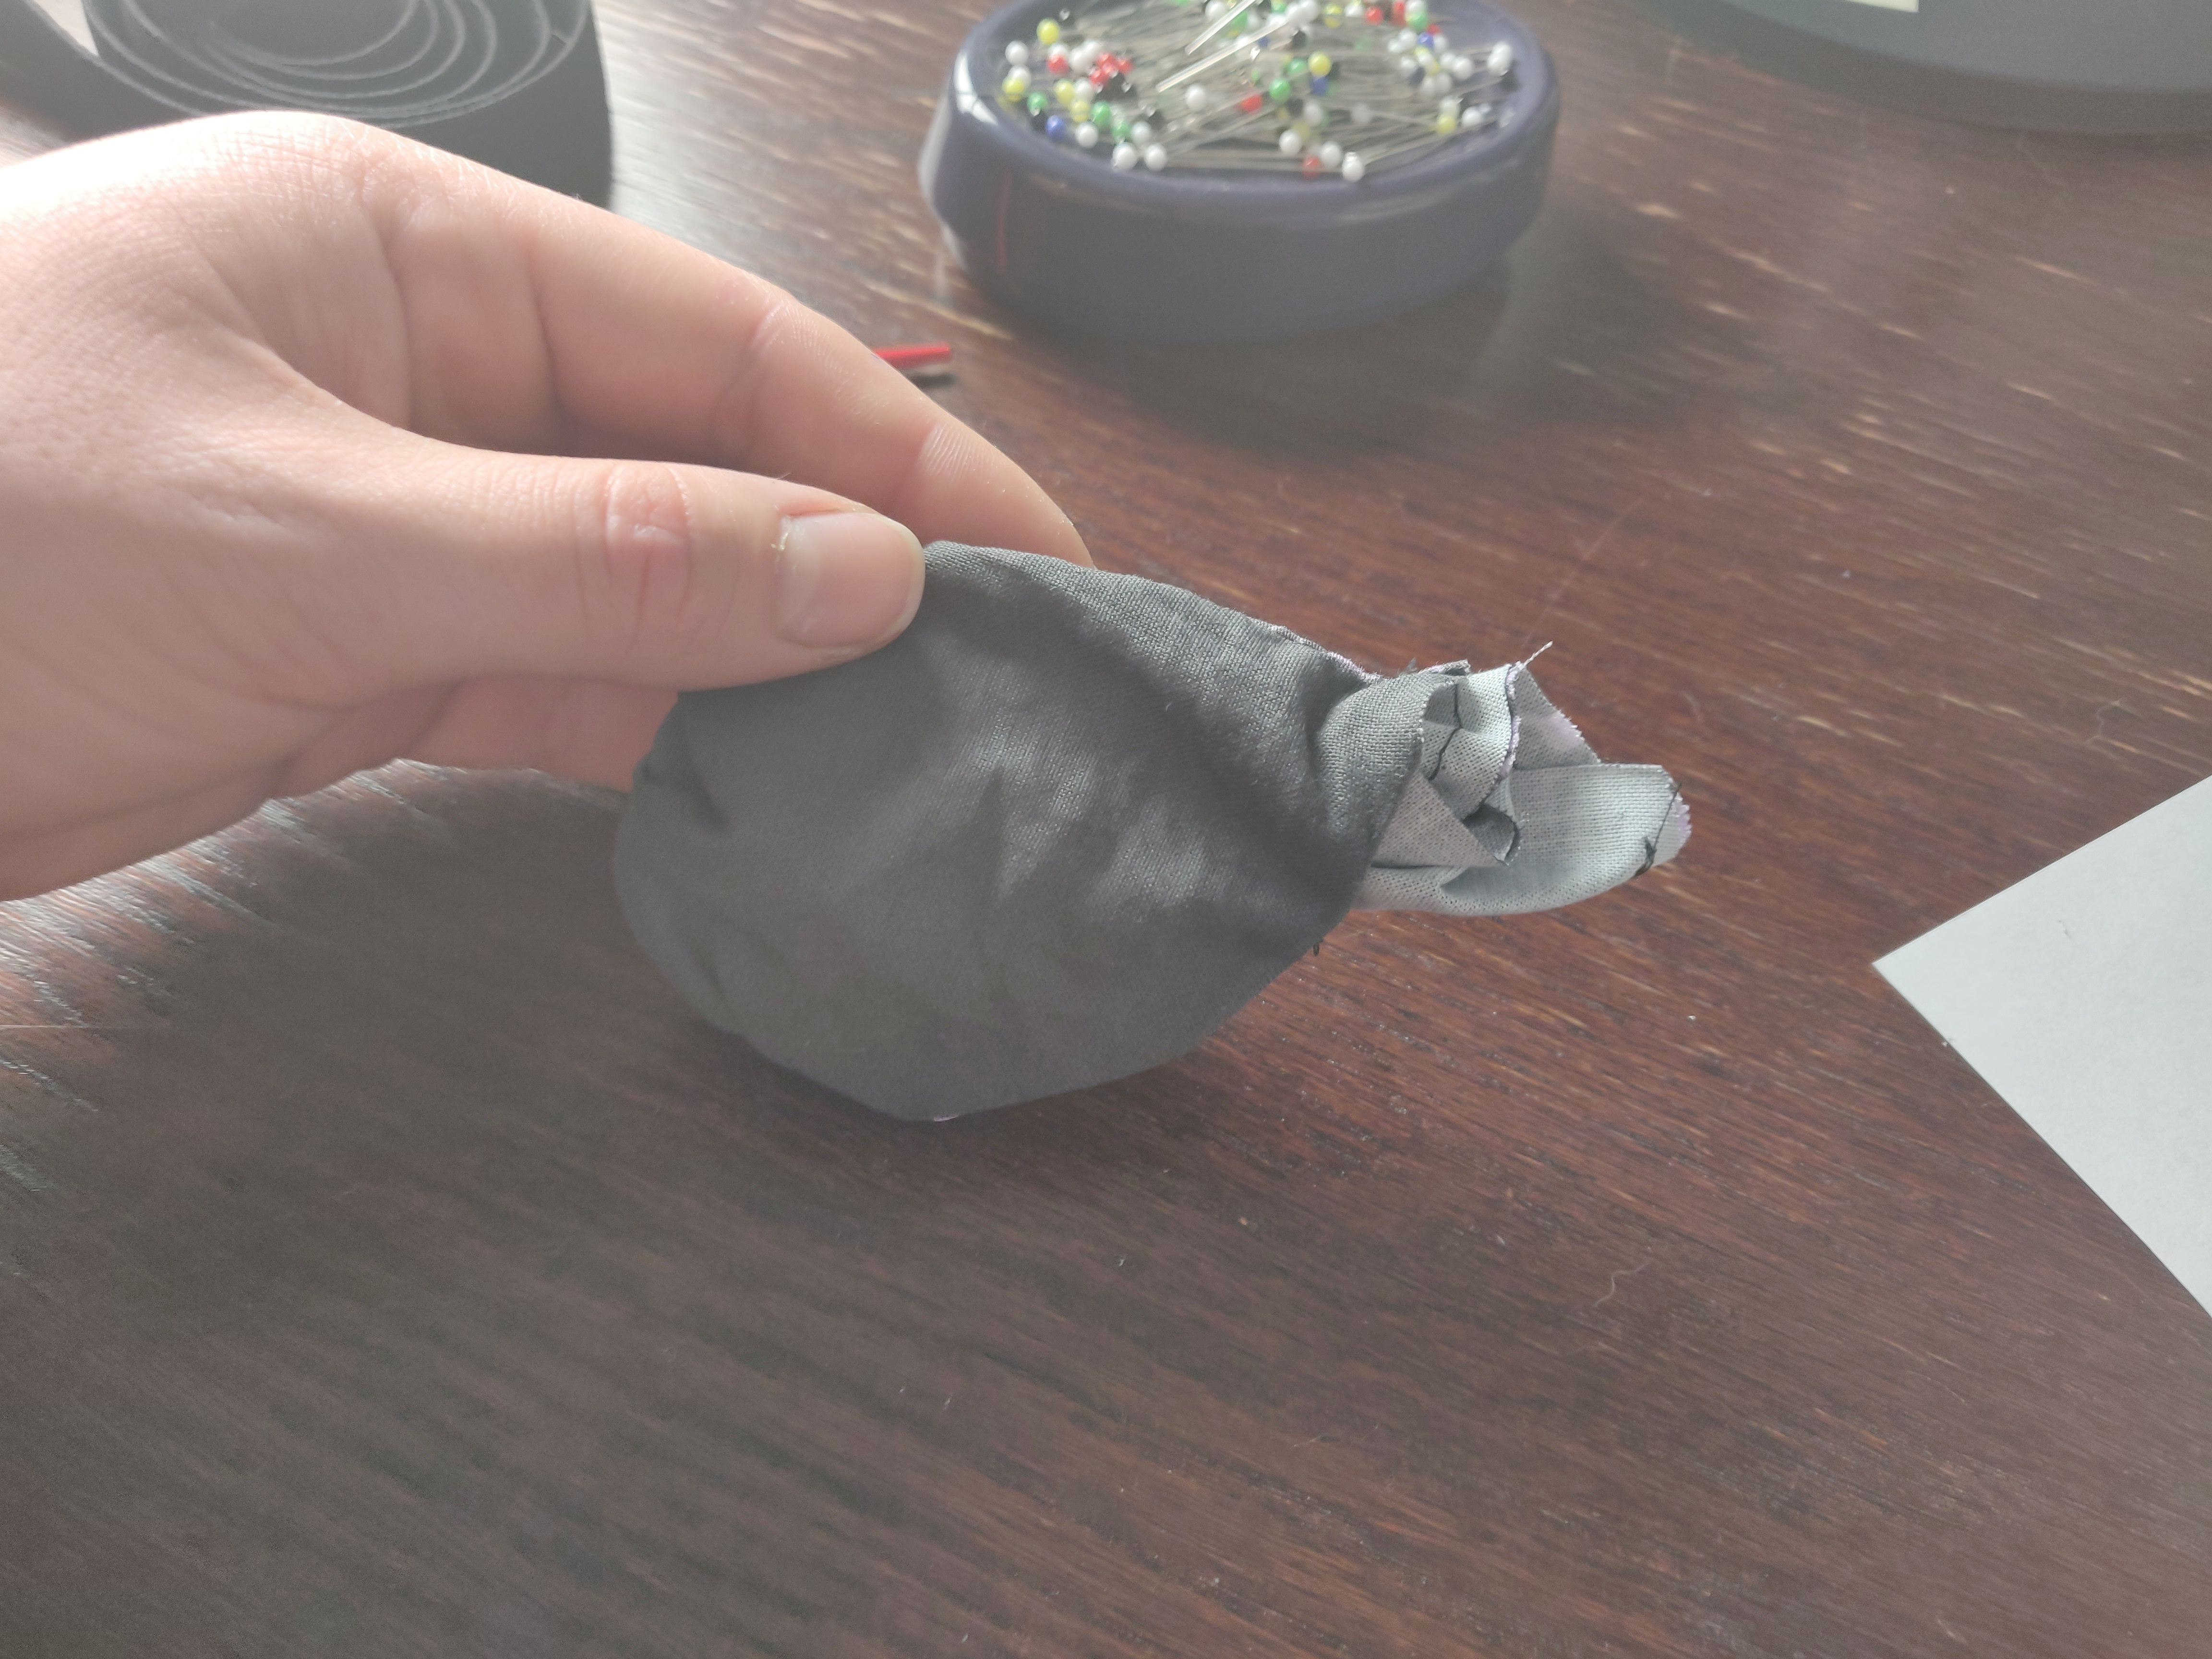
\includegraphics[width = \linewidth]{Pictures/07_Turning/Turning5.jpg}
        \caption{Die ganze Maske durchstecken}
        \label{Turning5}
    \end{subfigure}
    \begin{subfigure}{0.48\textwidth}
        \centering
        \includegraphics[width = \linewidth]{Pictures/07_Turning/Turning6.jpg}
        \caption{Fertig gewendete Maske}
        \label{Turning6}
    \end{subfigure}
    \caption{Wenden}
    \label{Turning}
\end{figure}

\section{Nasen-Befestigungen}
% Need a better name for this chapter
Der folgende Schritt ist der schwierigste und sollte sorgfältig durchgeführt werden. Man benötigt dafür den im ersten Schritt vorbereiteten Drahteinsatz und ein gleich langes Stück der Abdichtung (zum Beispiel aus halterlosen Strümpfen). Die beiden Materialien sind im Abbildung \ref{Nose01} zu sehen. Die Abdichtung ist ja dafür gedacht, das Rutschen zu verhindern, was allerdings für die Verarbeitung etwas schwierig ist. Damit das Material trotzdem mit der Nähmaschine verarbeitet werden kann und gut transportiert wird, kann man ein Stück Klopapier verwenden, das man auf die gummierte Seite legt (siehe Abbildung \ref{Nose02}). Das Klopapier wird einfach mit festgenäht und danach wieder entfernt.

\begin{figure}[ht]
    \vspace{0.5cm}
    \centering
    \begin{subfigure}{0.48\textwidth}
        \centering
        \includegraphics[width = \linewidth]{Pictures/09_NoseParts/NoseParts01.jpg}
        \caption{Drahteinsatz und Abdichtung}
        \label{Nose01}
    \end{subfigure}
    \begin{subfigure}{0.48\textwidth}
        \centering
        \includegraphics[width = \linewidth]{Pictures/09_NoseParts/NoseParts02.jpg}
        \caption{Abdichtung auf Klopapier}
        \label{Nose02}
    \end{subfigure}
    \caption{Vorbereitungen für die Nasen-Befestigungen}
    \label{NosePrep}
\end{figure}

Zuerst wird der vorbereitete Drahteinsatz zurechtgebogen, damit er besser zu positionieren ist (siehe Abbildung \ref{Nose03}). Dann wird er durch eine der Lücken ins innere der Maske, also zwischen Innen- und Außenstoff geschoben (siehe Abbildung \ref{Nose02}) und an die richtige Stelle an die spitze Seite der Maske positioniert. Es ist wichtig, den Drahteinsatz ganz an die Kante der zu schieben. Er sollte mittig positioniert sein. Anschließend wird der Drahteinsatz mit mehreren Stecknadeln eng an der Kante festgesteckt (siehe Abbildung \ref{Nose03}). Hier sollte man unbedingt auf eine gute Positionierung achten. Jetzt wird die Abdichtung inklusive dem Klopapier an die Innenseite der Maske positioniert wie in Abbildung \ref{Nose04} zu sehen. Wenn sie richtig sitzt, wird sie ebenfalls mit mehreren Stecknadeln festgesteckt (siehe Abbildung \ref{Nose05}). Dieser Schritt ist etwas schwierig, aber es lohnt sich, es im Zweifel mehrmals zu versuchen, bis sowohl Drahteinsatz als auch Abdichtung richtig sitzen, damit die Maske am Ende auch gut funktioniert, bequem sitzt und an der Nase dicht ist. Wenn der Sitz beider Elemente zufriedenstellend ist, wird der Drahteinsatz vorsichtig gerade gebogen, ohne die Stecknadeln zu lösen. Anschießend wird eine Naht gesetzt, die beide Elemente mit der Maske verbindet. Die Naht sollte recht eng an dem Drahteinsatz sein damit der Stoff in den der Drahteinsatz eingenäht ist mit der Maske vernäht wird. Auf Abbildung \ref{Nose06} ist die fertige Naht von außen zu sehen.\par

Auf der Innenseite der Maske sollte die Abdichtung mit dem Klopapier angenäht sein, wie auf Abbildung \ref{Nose09} zu sehen. Man kann jetzt vorsichtig das Klopapier um die Naht herum abreißen. Das Ergebnis sollte Abbildung \ref{Nose10} ähneln. Wenn die Naht gut gesetzt wurde, sollte die Abdichtung gut an der Maske befestigt sein. Falls das nicht der Fall ist, kann man an einer oder zwei Stellen noch mit Nadel und Faden manuell ein paar Stiche machen, um die Abdichtung besser an der Maske zu befestigen. Eine zweite Naht mit der Maschine ist hier nicht so ratsam, da das von außen nicht so gut aussieht. 

\begin{figure}[hp]
    \vspace{0.5cm}
    \centering
    \begin{subfigure}{0.48\textwidth}
        \centering
        \includegraphics[width = \linewidth]{Pictures/09_NoseParts/NoseParts03.jpg}
        \caption{Drahteinsat zurechtbiegen}
        \label{Nose03}
    \end{subfigure}
    \begin{subfigure}{0.48\textwidth}
        \centering
        \includegraphics[width = \linewidth]{Pictures/09_NoseParts/NoseParts04.jpg}
        \caption{Drahteinsatz in die Maske stecken}
        \label{Nose04}
    \end{subfigure}
    \begin{subfigure}{0.48\textwidth}
        \centering
        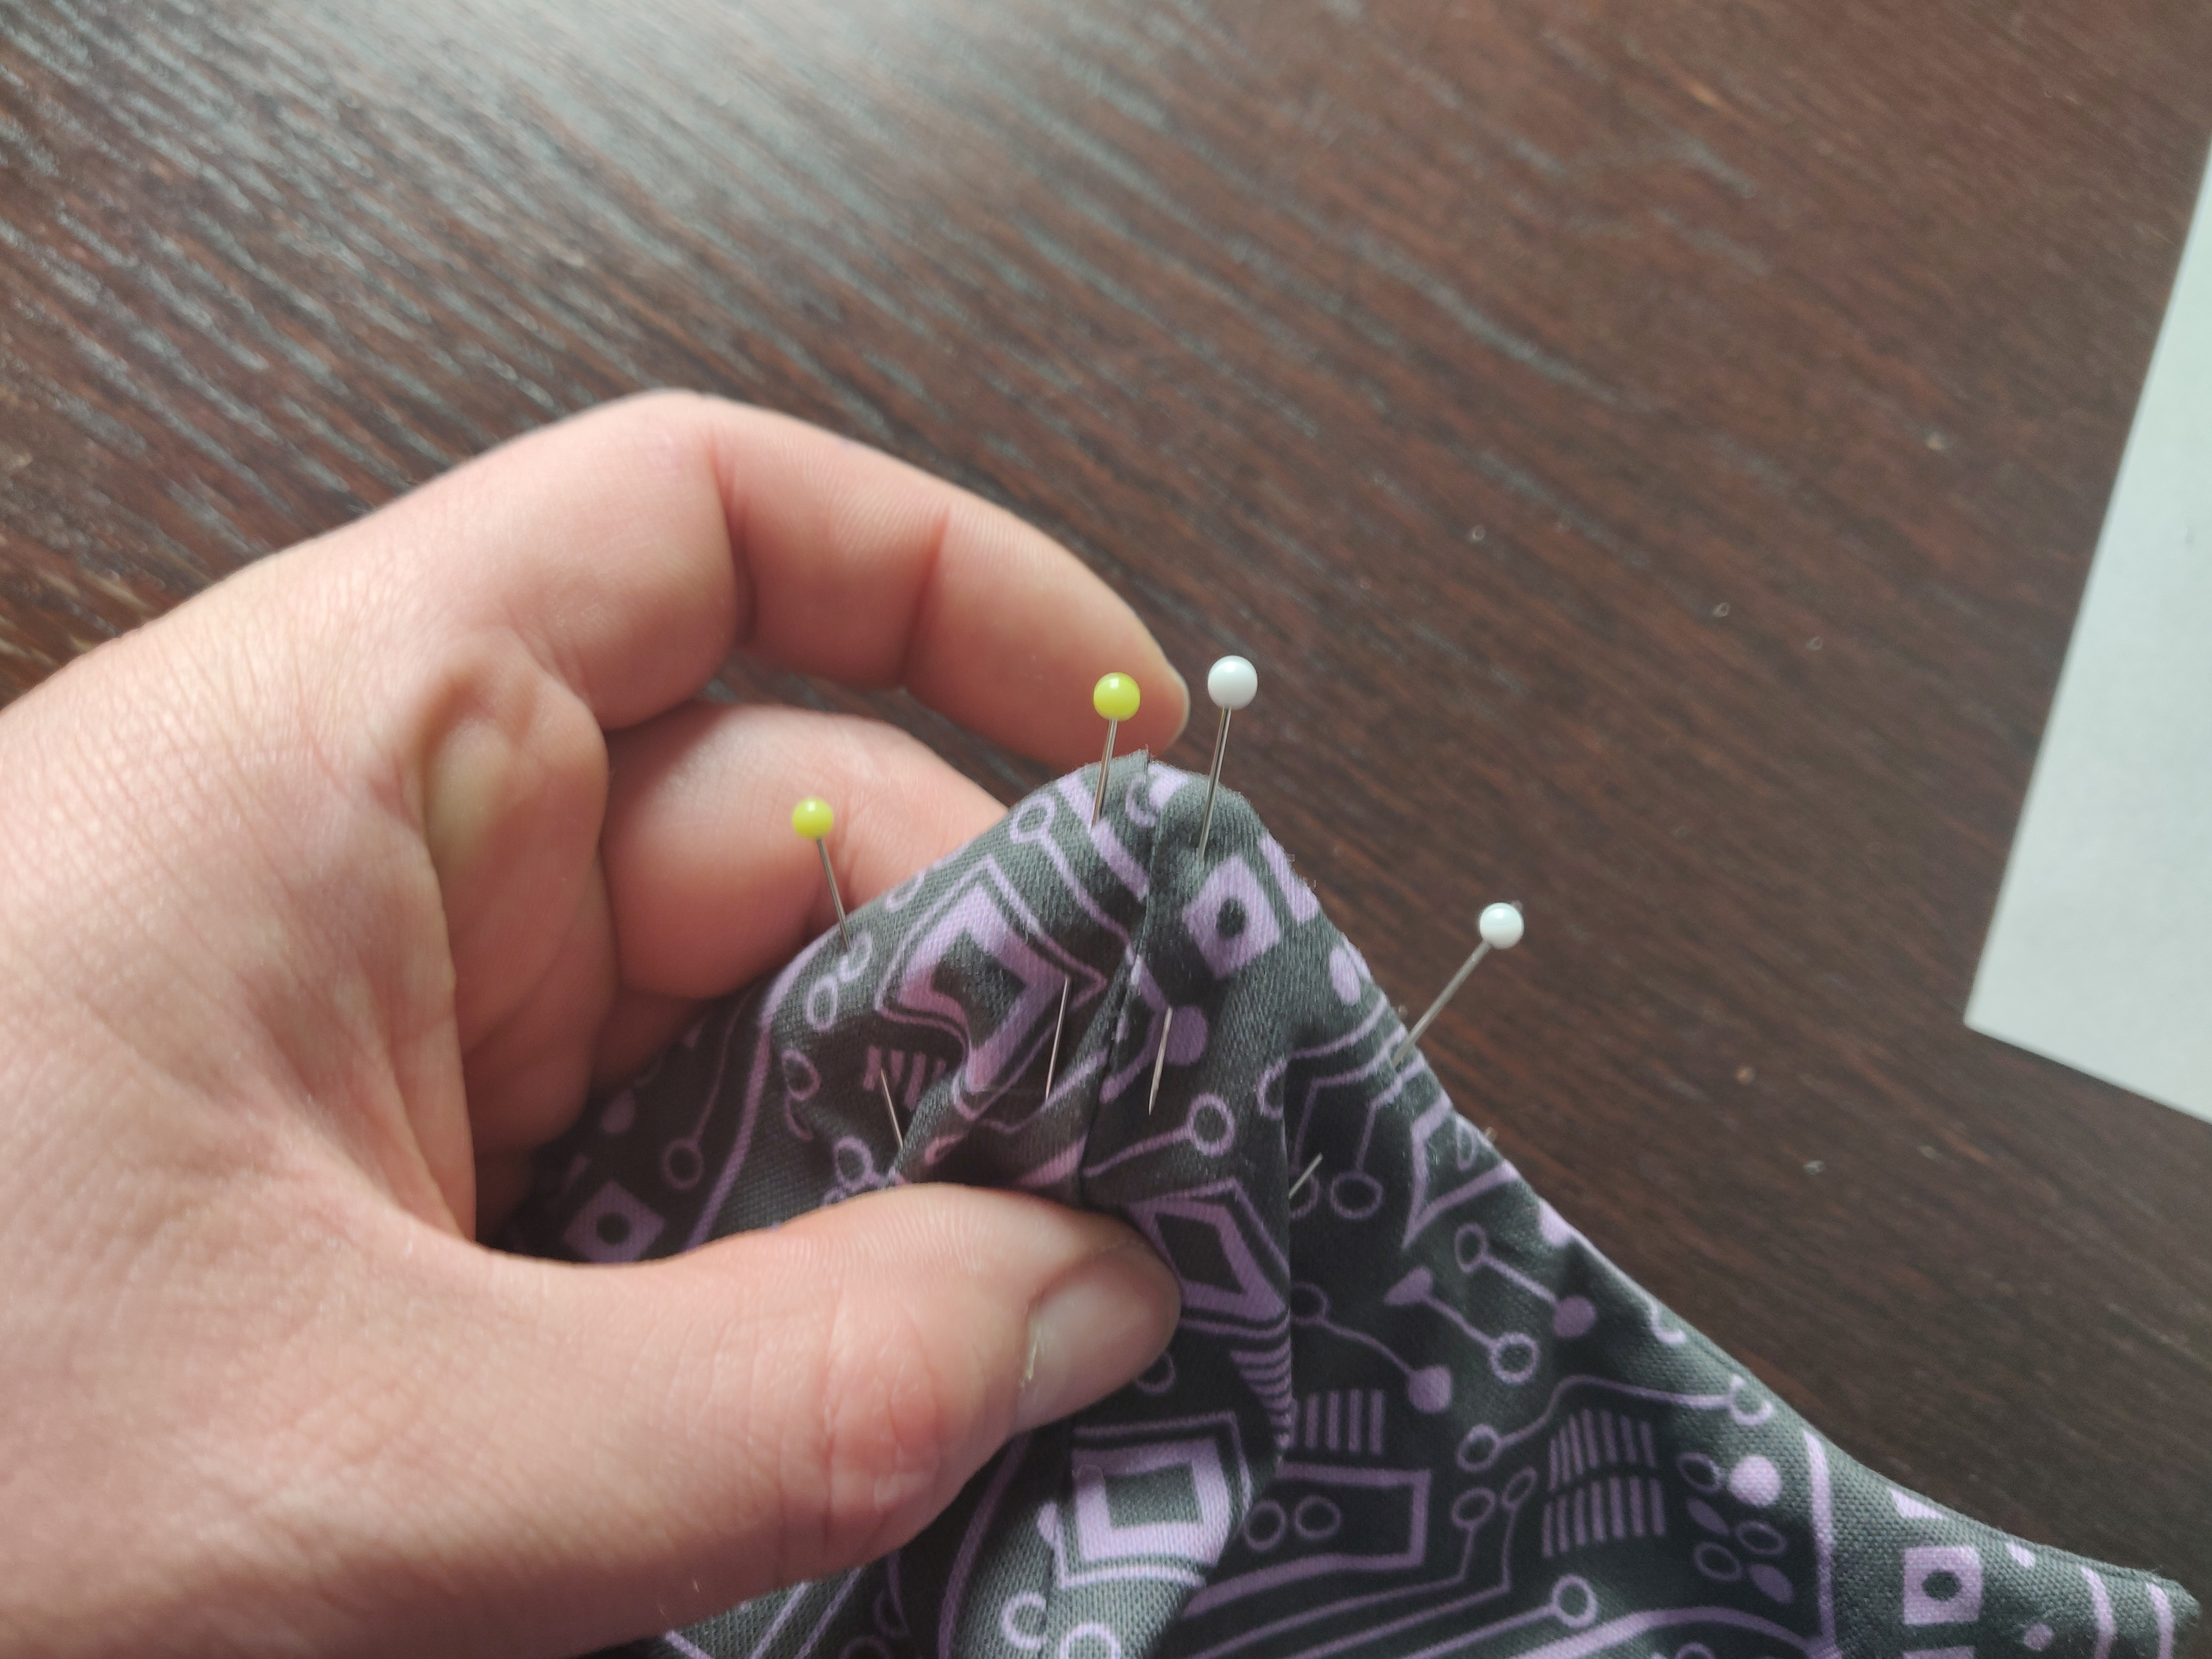
\includegraphics[width = \linewidth]{Pictures/09_NoseParts/NoseParts05.jpg}
        \caption{Drahteinsatz festecken}
        \label{Nose05}
    \end{subfigure}
    \begin{subfigure}{0.48\textwidth}
        \centering
        \includegraphics[width = \linewidth]{Pictures/09_NoseParts/NoseParts06.jpg}
        \caption{Abdichtung mit Klopapier positionieren}
        \label{Nose06}
    \end{subfigure}
    \begin{subfigure}{0.48\textwidth}
        \centering
        \includegraphics[width = \linewidth]{Pictures/09_NoseParts/NoseParts07.jpg}
        \caption{Beides feststecken}
        \label{Nose07}
    \end{subfigure}
    \begin{subfigure}{0.48\textwidth}
        \centering
        \includegraphics[width = \linewidth]{Pictures/09_NoseParts/NoseParts08.jpg}
        \caption{Nach der Naht}
        \label{Nose08}
    \end{subfigure}
    \caption{Nasen-Befestigung}
    \label{NoseMain}
\end{figure}


\begin{figure}[ht]
    \vspace{0.5cm}
    \centering
    \begin{subfigure}{0.48\textwidth}
        \centering
        \includegraphics[width = \linewidth]{Pictures/09_NoseParts/NoseParts09.jpg}
        \caption{Fertige Naht von innen}
        \label{Nose09}
    \end{subfigure}
    \begin{subfigure}{0.48\textwidth}
        \centering
        \includegraphics[width = \linewidth]{Pictures/09_NoseParts/NoseParts10.jpg}
        \caption{Nach Entfernung des Klopapier}
        \label{Nose10}
    \end{subfigure}
    \caption{Abdichtung nach der Befestigung}
    \label{NoseRes}
\end{figure}

\section{Nackenband}
Im folgenden Schritt wird das Nackenband an der Maske angenäht. Das Band wird am oberen der Ende der Seite der Maske positioniert, wie in Abbildung \ref{Strap1} zu sehen. Allerdings wird das Band in die vorhandenen Öffnungen an der Seite der Maske gesteckt, die man in den vorherigen Schritten offen gelassen hat. Das Band wird etwa ein bis zwei Zentimeter tief in die Maske (zwischen Außenstoff und Innenstoff) gesteckt und dort mit zwei Stecknadeln festgesteckt (siehe Abbildung \ref{Strap2}). Die Länge der Bäder sollte man vorher dadurch festlegen, dass man die Maske anprobiert. Beispiellängen sind auf den Abbildungen zu sehen, das Band sollte lieber zu lang als zu kurz sein. Das gleiche macht man auf der anderen Seite (siehe Abbildung \ref{Strap3}). Dann setzt man jeweils eine Naht an dieser Stelle, die gleichzeitig das Nackenband befestigt und die obere Öffnung schließt. An dieser Stelle sollte man ruhig öfter hin und her nähen, um eine wirklich stabile Naht zu erzeugen. Das Ergebnis ist in Abbildung \ref{Strap4} zu sehen. 

\begin{figure}[ht]
    \vspace{0.5cm}
    \centering
    \begin{subfigure}{0.48\textwidth}
        \centering
        \includegraphics[width = \linewidth]{Pictures/10_Straps/Straps1.jpg}
        \caption{Positionierung des Bandes}
        \label{Strap1}
    \end{subfigure}
    \begin{subfigure}{0.48\textwidth}
        \centering
        \includegraphics[width = \linewidth]{Pictures/10_Straps/Straps2.jpg}
        \caption{Feststecken erstes Band}
        \label{Strap2}
    \end{subfigure}
    \begin{subfigure}{0.48\textwidth}
        \centering
        \includegraphics[width = \linewidth]{Pictures/10_Straps/Straps3.jpg}
        \caption{Feststecken zweites Band}
        \label{Strap3}
    \end{subfigure}
    \begin{subfigure}{0.48\textwidth}
        \centering
        \includegraphics[width = \linewidth]{Pictures/10_Straps/Straps4.jpg}
        \caption{Fertig angenähtes Nakenband}
        \label{Strap4}
    \end{subfigure}
    \caption{Nackenband}
    \label{Strap}
\end{figure}

\section{Faltung}
Im nächsten Schritt wird die Maske individuell an die eigene Gesichtsform angepasst. Dazu sollte man die Maske das erste mal anziehen, so wie man sie später auch tragen wird. Die beiden Bänder kann man im Nacken mit einer Sicherheitsnadel aneinander befestigen. Dann faltet man die abstehenden unteren Ecken der Maske nach oben, wie in den Abbildungen \ref{Folding1} und \ref{Folding2} zu sehen. Man fixiert die Faltung wie in Abbildung \ref{Folding3} und steckt sie vorsichtig mit einer Stecknadel fest wie in Abbildung \ref{Folding4}. Das Vorgehen führt man auf beiden Seiten gleich durch, dabei sollte man auch auf Symmetrie achten. Dann zieht man die Maske vorsichtig wieder aus und kann die Faltung gegebenenfalls nochmal korrigieren (siehe Abbildung \ref{Folding5}). Anschließend fixiert man die Faltung mit einer Naht so wie in Abbildung \ref{Folding6} zu sehen. 

\begin{figure}[hp]
    \vspace{0.5cm}
    \centering
    \begin{subfigure}{0.48\textwidth}
        \centering
        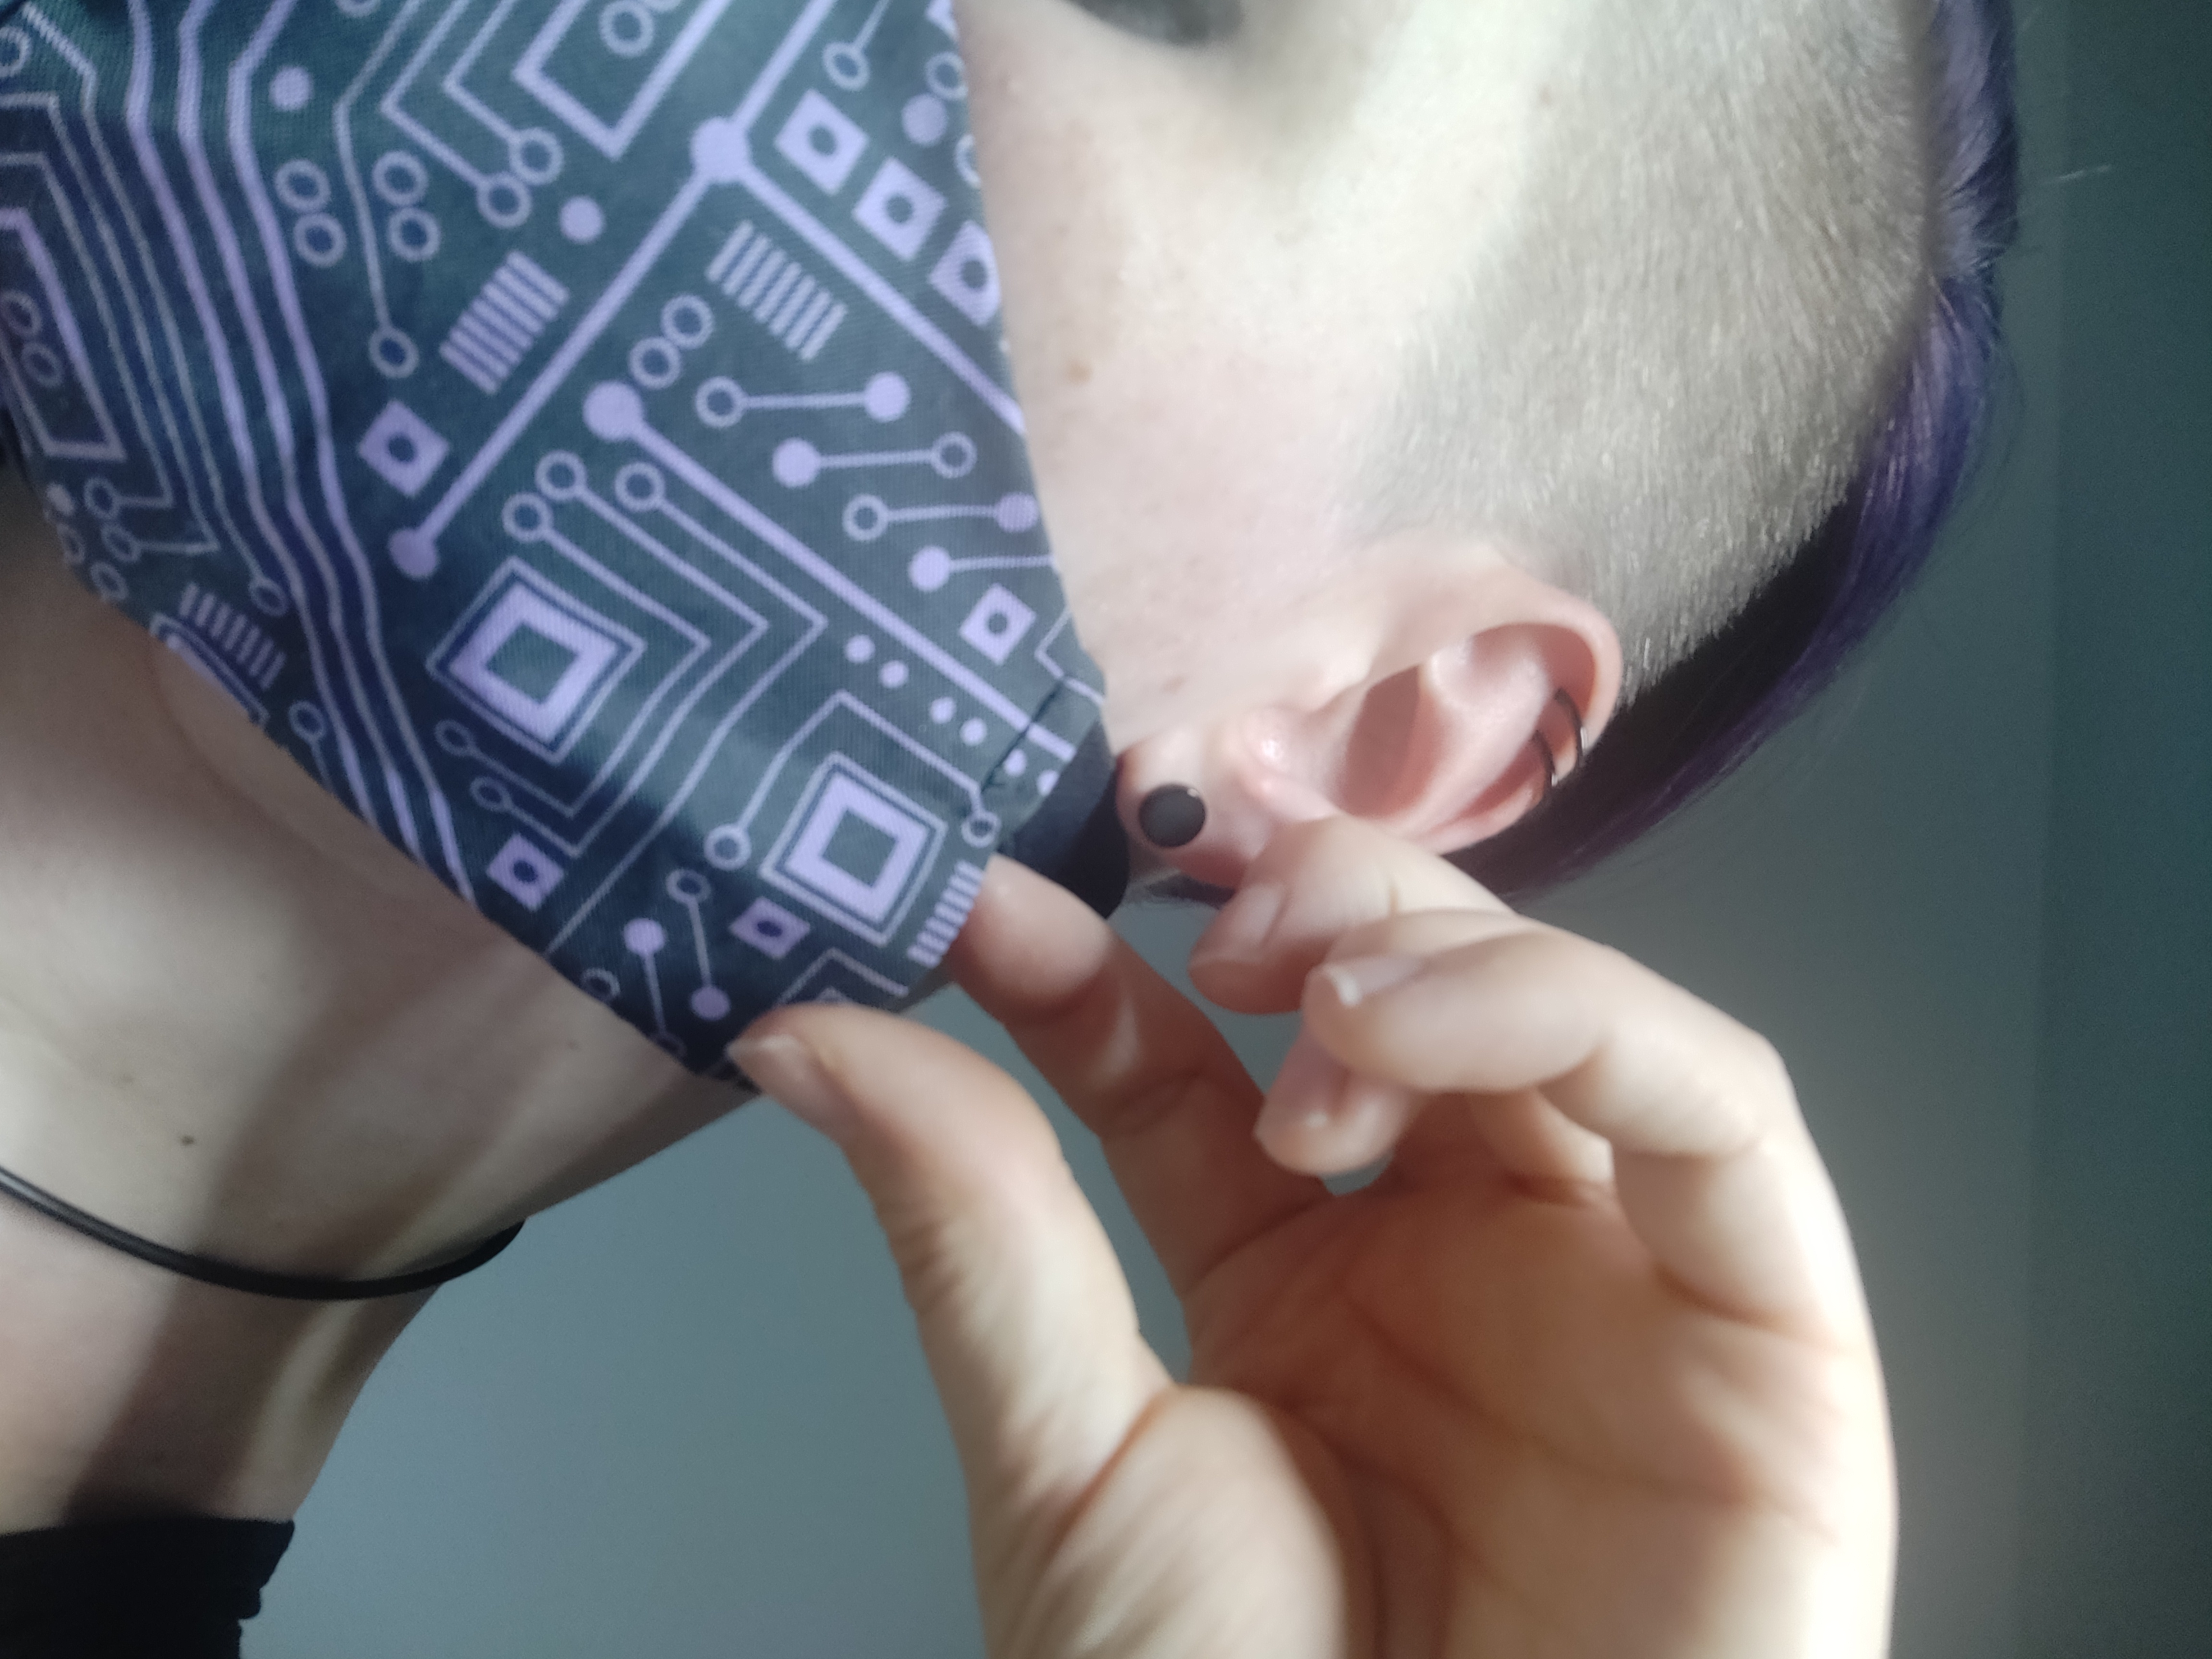
\includegraphics[width = \linewidth]{Pictures/11_Folding/Folding1.jpg}
        \caption{Faltung ansetzen}
        \label{Folding1}
    \end{subfigure}
    \begin{subfigure}{0.48\textwidth}
        \centering
        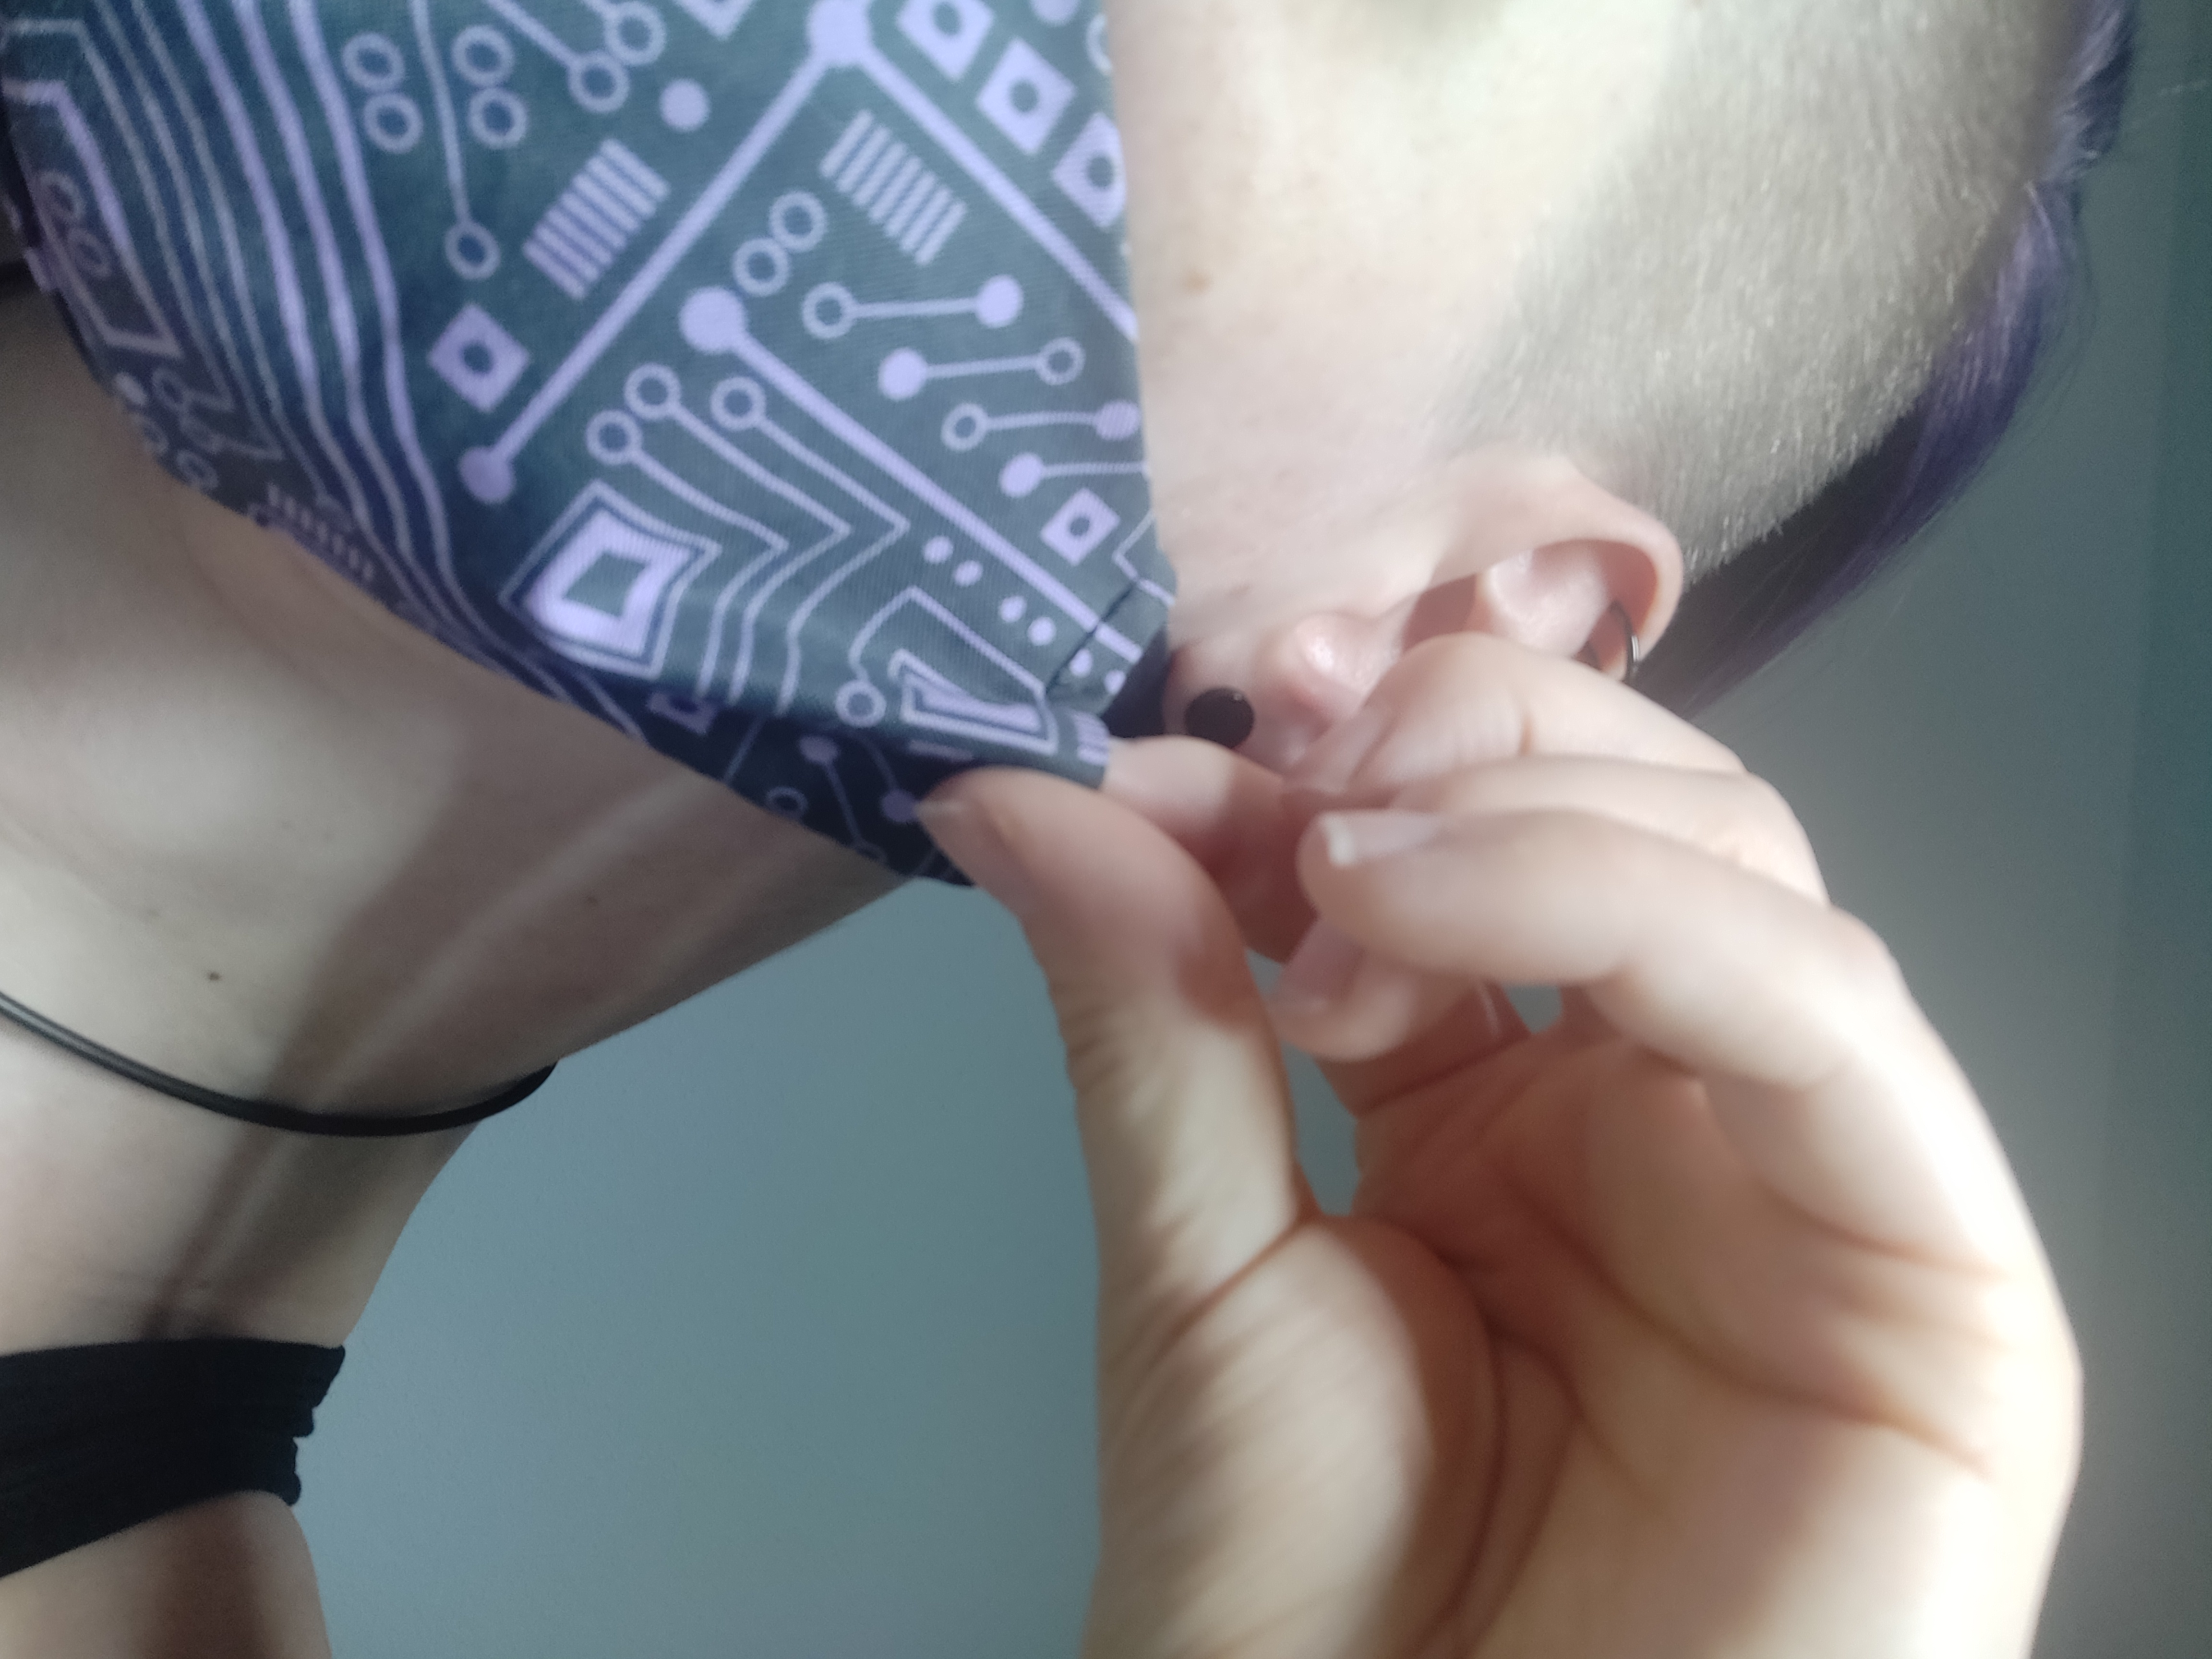
\includegraphics[width = \linewidth]{Pictures/11_Folding/Folding2.jpg}
        \caption{Faltung legen}
        \label{Folding2}
    \end{subfigure}
    \begin{subfigure}{0.48\textwidth}
        \centering
        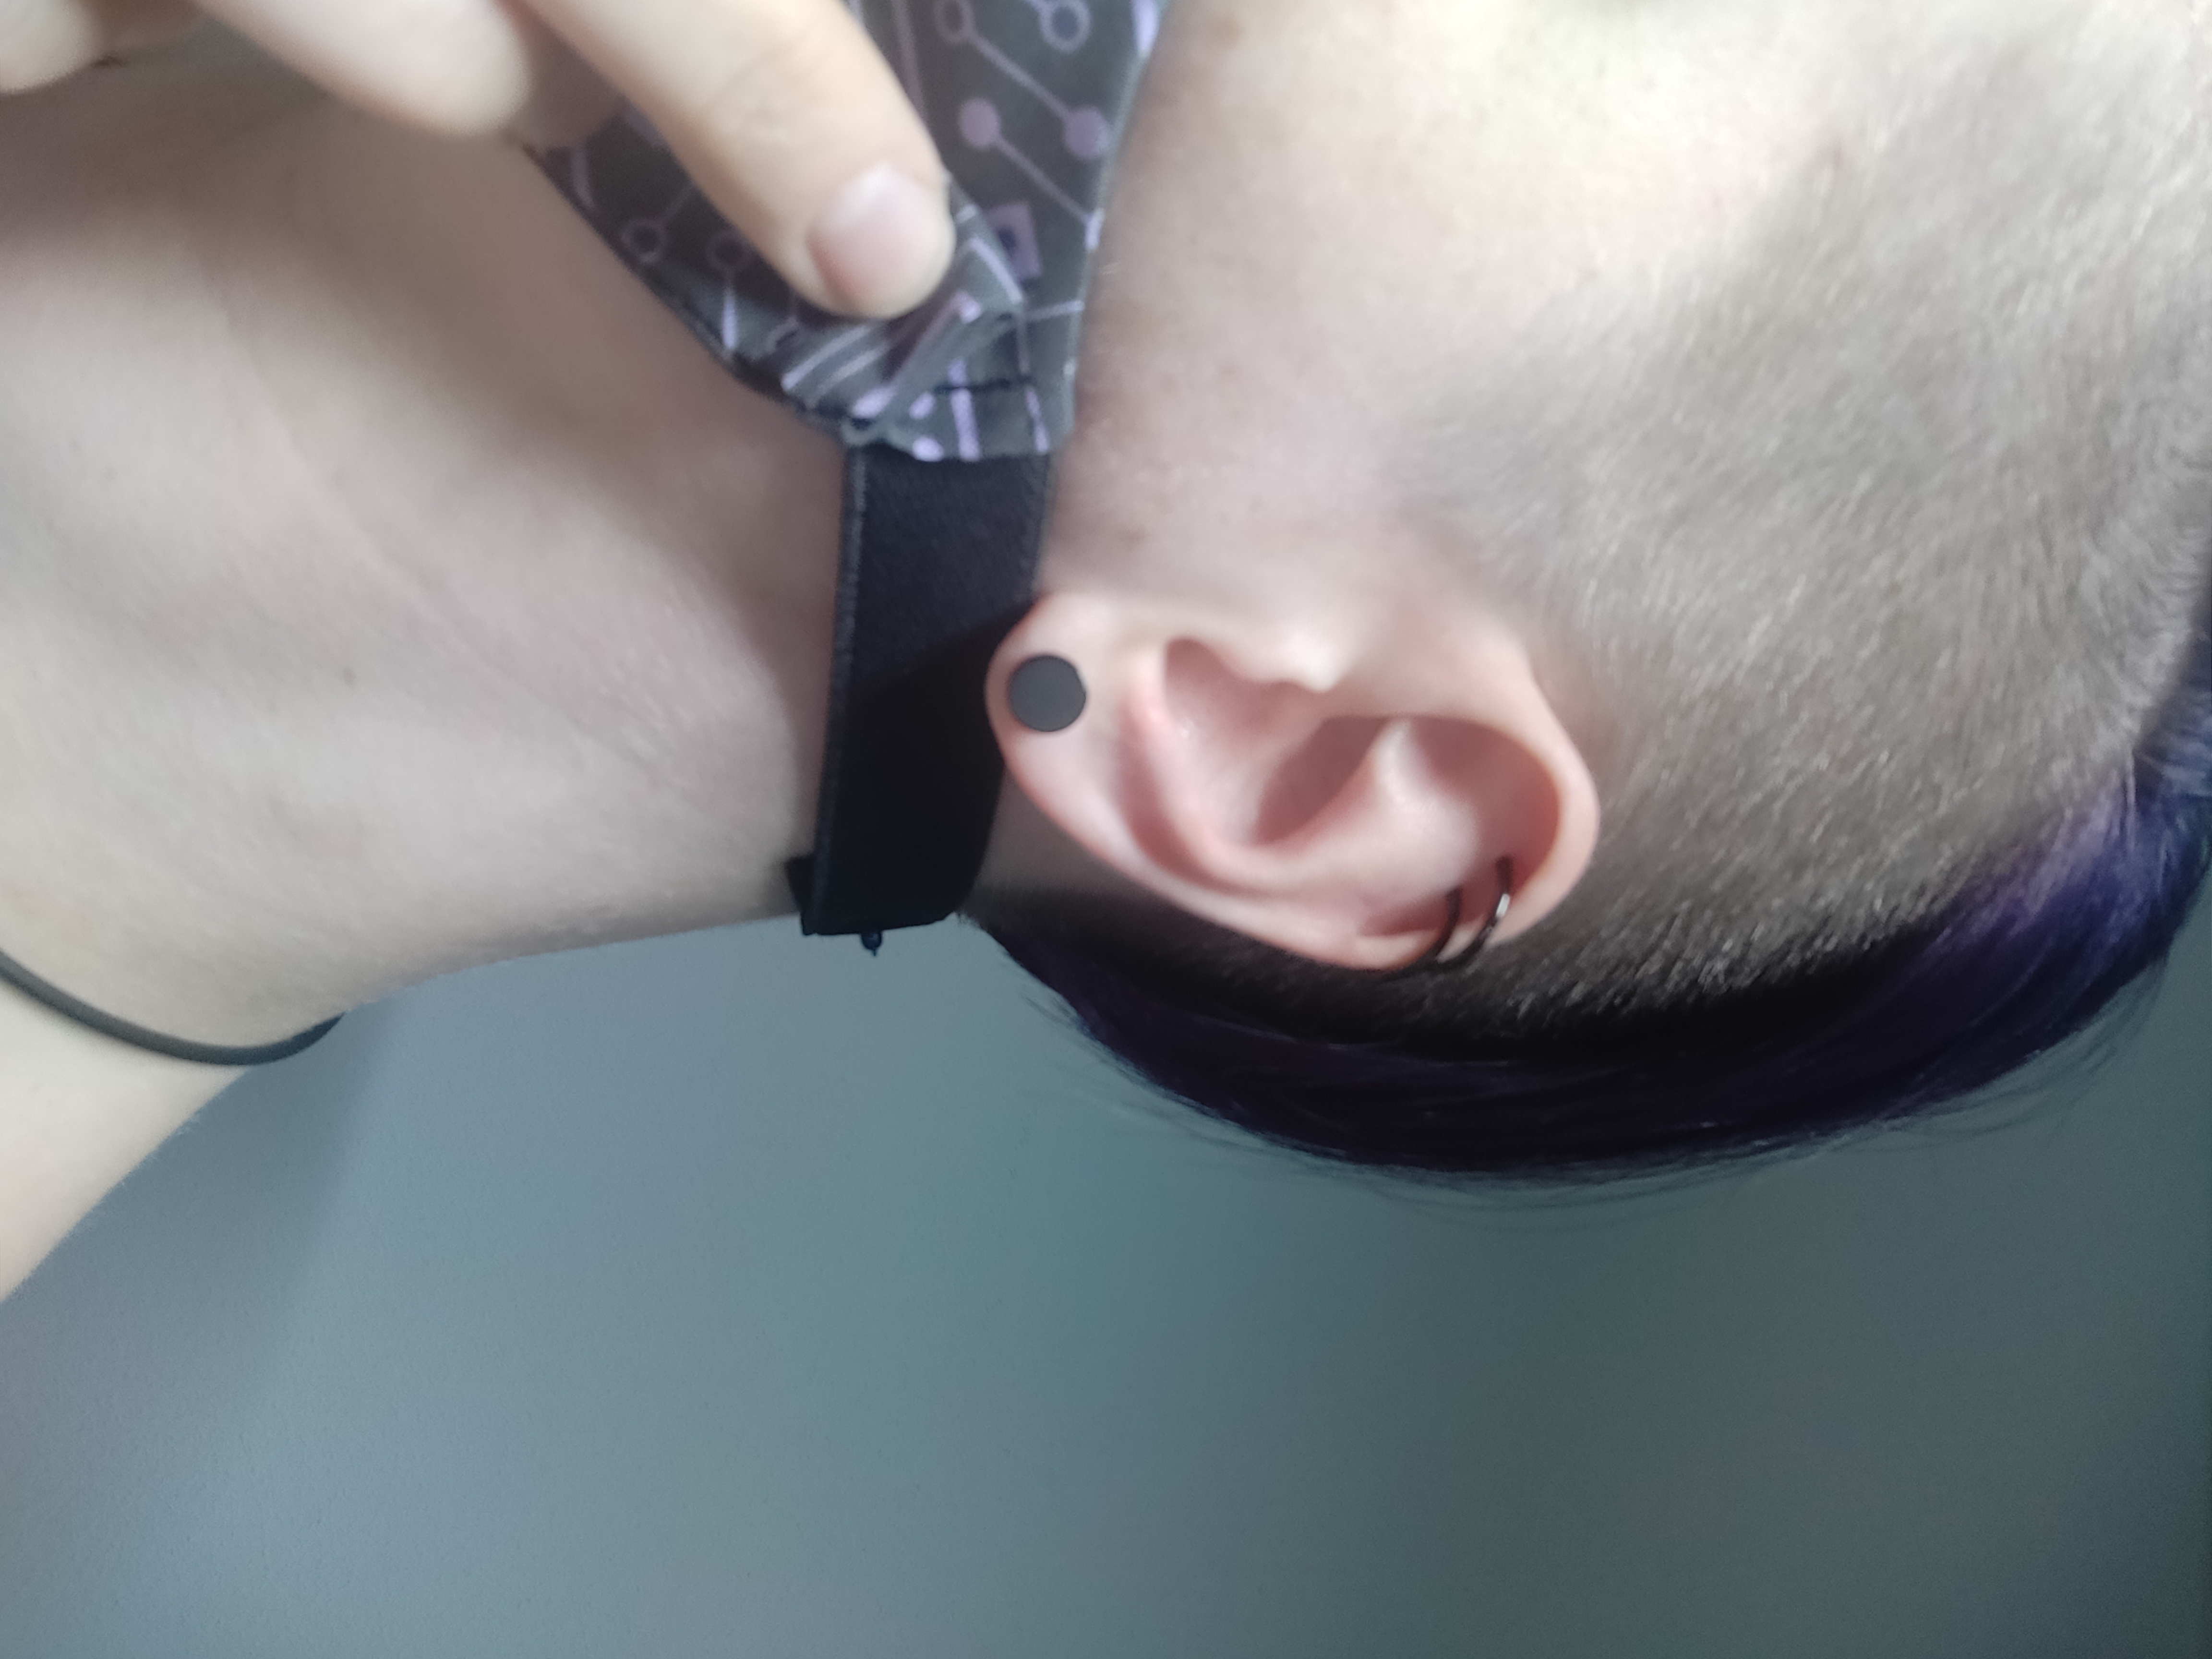
\includegraphics[width = \linewidth]{Pictures/11_Folding/Folding3.jpg}
        \caption{Fertige Faltung}
        \label{Folding3}
    \end{subfigure}
    \begin{subfigure}{0.48\textwidth}
        \centering
        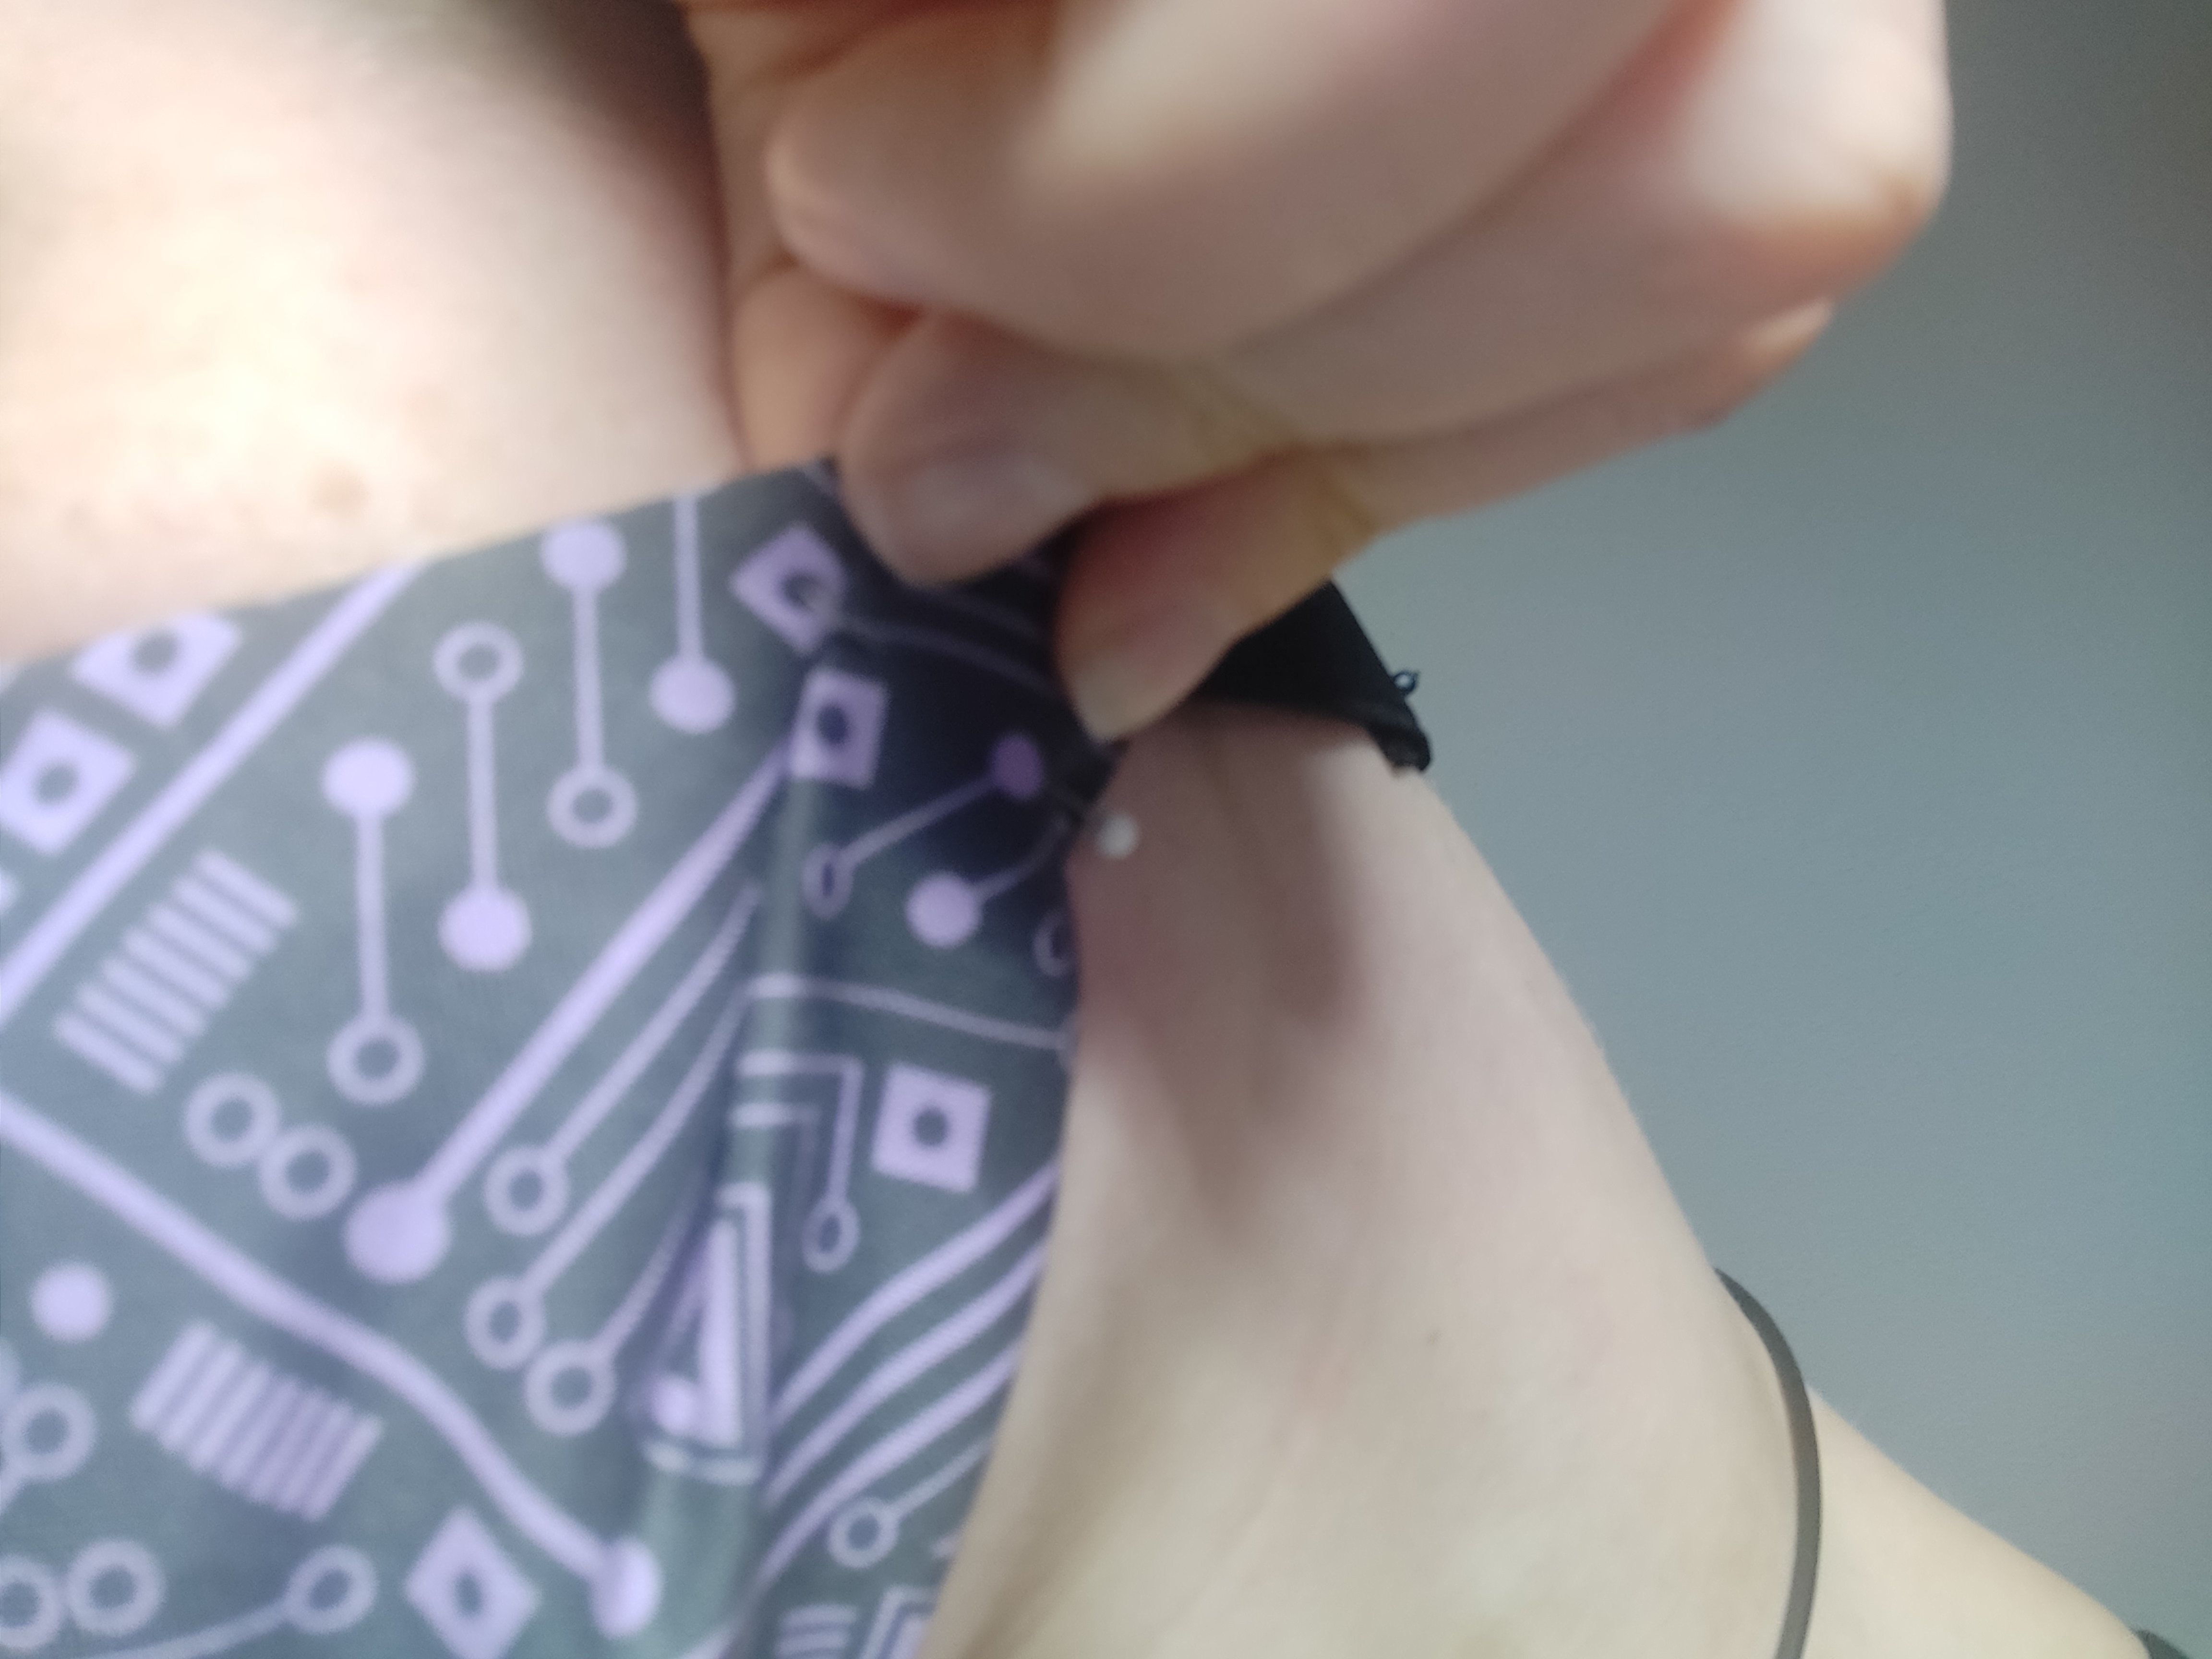
\includegraphics[width = \linewidth]{Pictures/11_Folding/Folding4.jpg}
        \caption{Faltung feststecken}
        \label{Folding4}
    \end{subfigure}
    \begin{subfigure}{0.48\textwidth}
        \centering
        \includegraphics[width = \linewidth]{Pictures/11_Folding/Folding5.jpg}
        \caption{Festgesteckte Faltung}
        \label{Folding5}
    \end{subfigure}
    \begin{subfigure}{0.48\textwidth}
        \centering
        \includegraphics[width = \linewidth]{Pictures/11_Folding/Folding6.jpg}
        \caption{Angenähte Faltung}
        \label{Folding6}
    \end{subfigure}
    \caption{Faltung}
    \label{Folding}
\end{figure}

\clearpage
\section{Verschluss}
Die Maske ist jetzt fast fertig, im letzten Schritt wird der Verschluss angebracht. Dafür gibt es verschiedene Möglichkeiten, beispielsweise Klett oder Druckknopf wie in Abbildung \ref{Fastener1}. Auch normale Knöpfe, Magnete oder ganz andere Verschlüsse sind denkbar. Der Vorteil an Klett ist der geringe Aufwand und die stufenlose Verstellbarkeit. Es kann Klett mit Kleberückseite verwendet werden, allerdings sollten noch zusätzlich zwei Nähte pro Klett gesetzet werden, um es sicher zu befestigen. Das befestigte Klett ist in Abbildung \ref{Fastener2} zu sehen. Der Verschluss sollte so befestigt werden, dass die Maske zwar so eng sitzt, dass sie oben fest abschließt, aber nicht so fest, dass sie auf Dauer drückt.

\begin{figure}[ht]
    \vspace{0.5cm}
    \centering
    \begin{subfigure}{0.48\textwidth}
        \centering
        \includegraphics[width = \linewidth]{Pictures/12_Fastener/Fastener1.jpg}
        \caption{Fertige Naht von innen}
        \label{Fastener1}
    \end{subfigure}
    \begin{subfigure}{0.48\textwidth}
        \centering
        \includegraphics[width = \linewidth]{Pictures/12_Fastener/Fastener2.jpg}
        \caption{Nach Entfernung des Klopapier}
        \label{Fastener2}
    \end{subfigure}
    \caption{Abdichtung nach der Befestigung}
    \label{Fastener}
\end{figure}

\vspace{0.2cm}
Der Mund-Nasen-Schutz ist fertig! Er kann jetzt getragen und eingesetzt werden.

\begin{figure}
    \centering
    \includegraphics[width = 0.5\textwidth]{Pictures/00_Completed/Gesamt2.jpg}
    \label{Ready}
\end{figure}

\end{document}
